\subsectionaddtolist{گزارش مراحل کار}
در توسعه پروژه Mini-NginX ، مراحل کار به صورت زیر دنبال شد تا یک سرور HTTP سبک و قابل تنظیم پیاده‌سازی شود. 

\begin{enumerate}
    \item \textbf{مرحله برنامه‌ریزی و طراحی:} ابتدا نیازهای پروژه تعریف شد، شامل پشتیبانی از تنظیمات \lr{YAML} ، انواع مسیرها (ریدایرکت، سرو فایل، پروکسی معکوس، سرو دایرکتوری) و استفاده از الگوی استراتژی برای هندلرها. معماری لایه‌ای انتخاب شد تا نگرانی‌ها جدا شوند.
    
    \item \textbf{پیاده‌سازی بارگذاری تنظیمات:} فایل \texttt{config.go} نوشته شد برای خواندن فایل \lr{YAML} و تبدیل به ساختار داده‌ای. این شامل تعریف \lr{struct} های \lr{Config} و \lr{Route} بود.
    
    \item \textbf{پیاده‌سازی سرور و مدیریت اتصالات:} در \texttt{server.go}، \lr{listener TCP} روی پورت مشخص ایجاد شد و برای هر اتصال ورودی یک goroutine اختصاص یافت تا concurrency پشتیبانی شود.
    
    \item \textbf{پیاده‌سازی روتینگ و دیسپچ:} در \texttt{router.go}، پارسر خط درخواست اضافه شد، مسیرها با استفاده از پیشوند تطبیق داده شدند و با switch بر اساس نوع مسیر، دیسپچ به هندلر انجام شد.
    
    \item \textbf{پیاده‌سازی هندلرها:} چهار هندلر مستقل نوشته شد: \lr{Redirect}، StaticFile، ServeDir، \lr{ReverseProxy}. هر کدام با استراتژی ساده پیاده‌سازی شدند.
    
    \item \textbf{افزودن ویژگی‌های کمکی:} لاگینگ به فایل و کنسول اضافه شد، و تست دستی با ابزارهایی مانند curl انجام شد.
    
\end{enumerate}


\subsectionaddtolist{بررسی صحت عملکرد برنامه}

در ابتدا کانفیگ \lr{YAML} به صورت زیر تعریف شد:


\begin{center}
    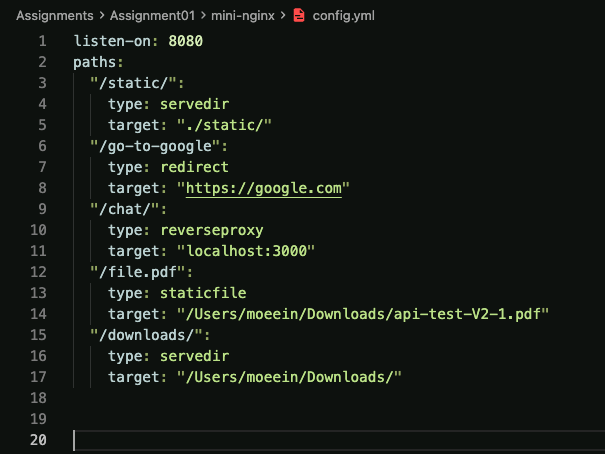
\includegraphics[width=0.5\textwidth]{figs/config-yml.png}
\end{center}

این کانفیگ از قابلیت‌های زیر پشتیبانی می‌کند:

\begin{itemize}
    \item Serverdir
    \item StaticFile
    \item ReverseProxy
    \item Redirect
\end{itemize}

سپس با استفاده از دستور زیر، برنامه‌را اجرا می‌کنیم:

\begin{center}
    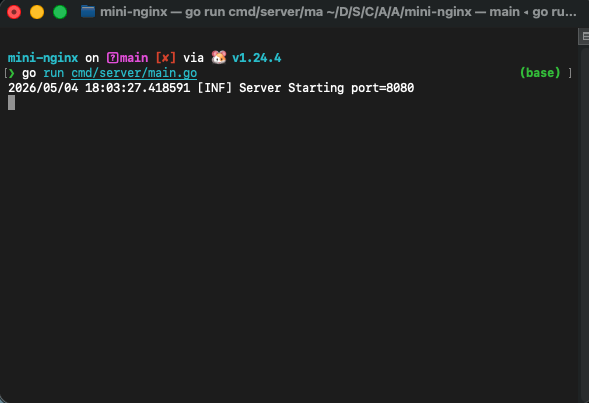
\includegraphics[width=0.5\textwidth]{figs/image.png}
\end{center}

تست کردن \lr{Redirect} با استفاده از Curl:

\begin{center}
    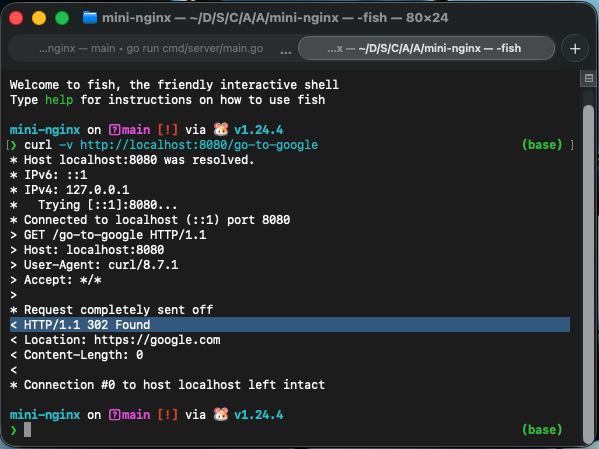
\includegraphics[width=0.5\textwidth]{figs/image2.png}
\end{center}

حال یک سرور \lr{http python} روی پورت \lr{3000}
بالا میاوریم تا ببینیم \lr{ReverseProxy} درست کار می‌کند یا نه:

\begin{center}
    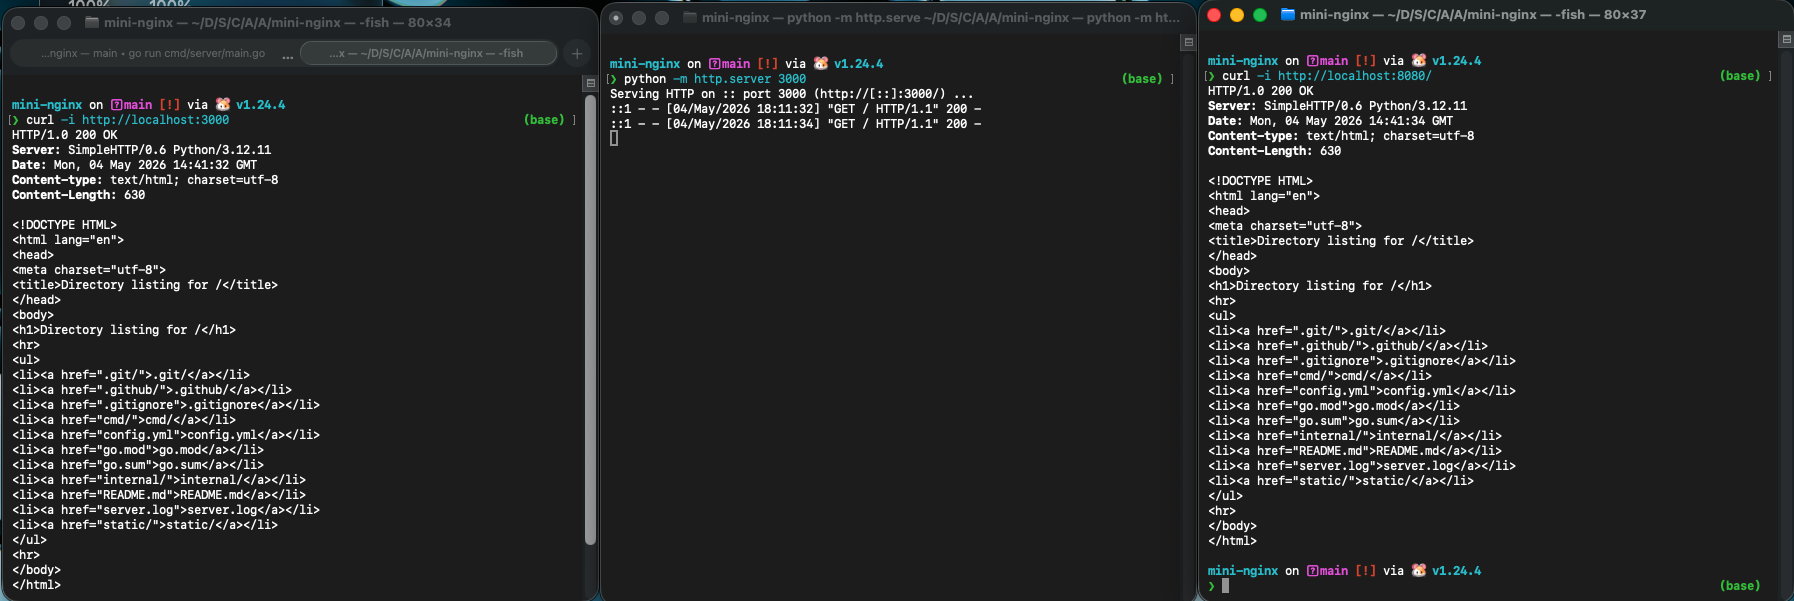
\includegraphics[width=1\textwidth]{figs/image3.png}
\end{center}

همانطور که مشخص است، درخواست مستقیم و درخواست به وب‌سرور \lr{Mini-NginX} هر دو یک نتیجه را دارند.

در نهایت قابلیت سرو کردن دایرکتوری و فایل‌های استاتیک را تست می‌کنیم:


\begin{center}
    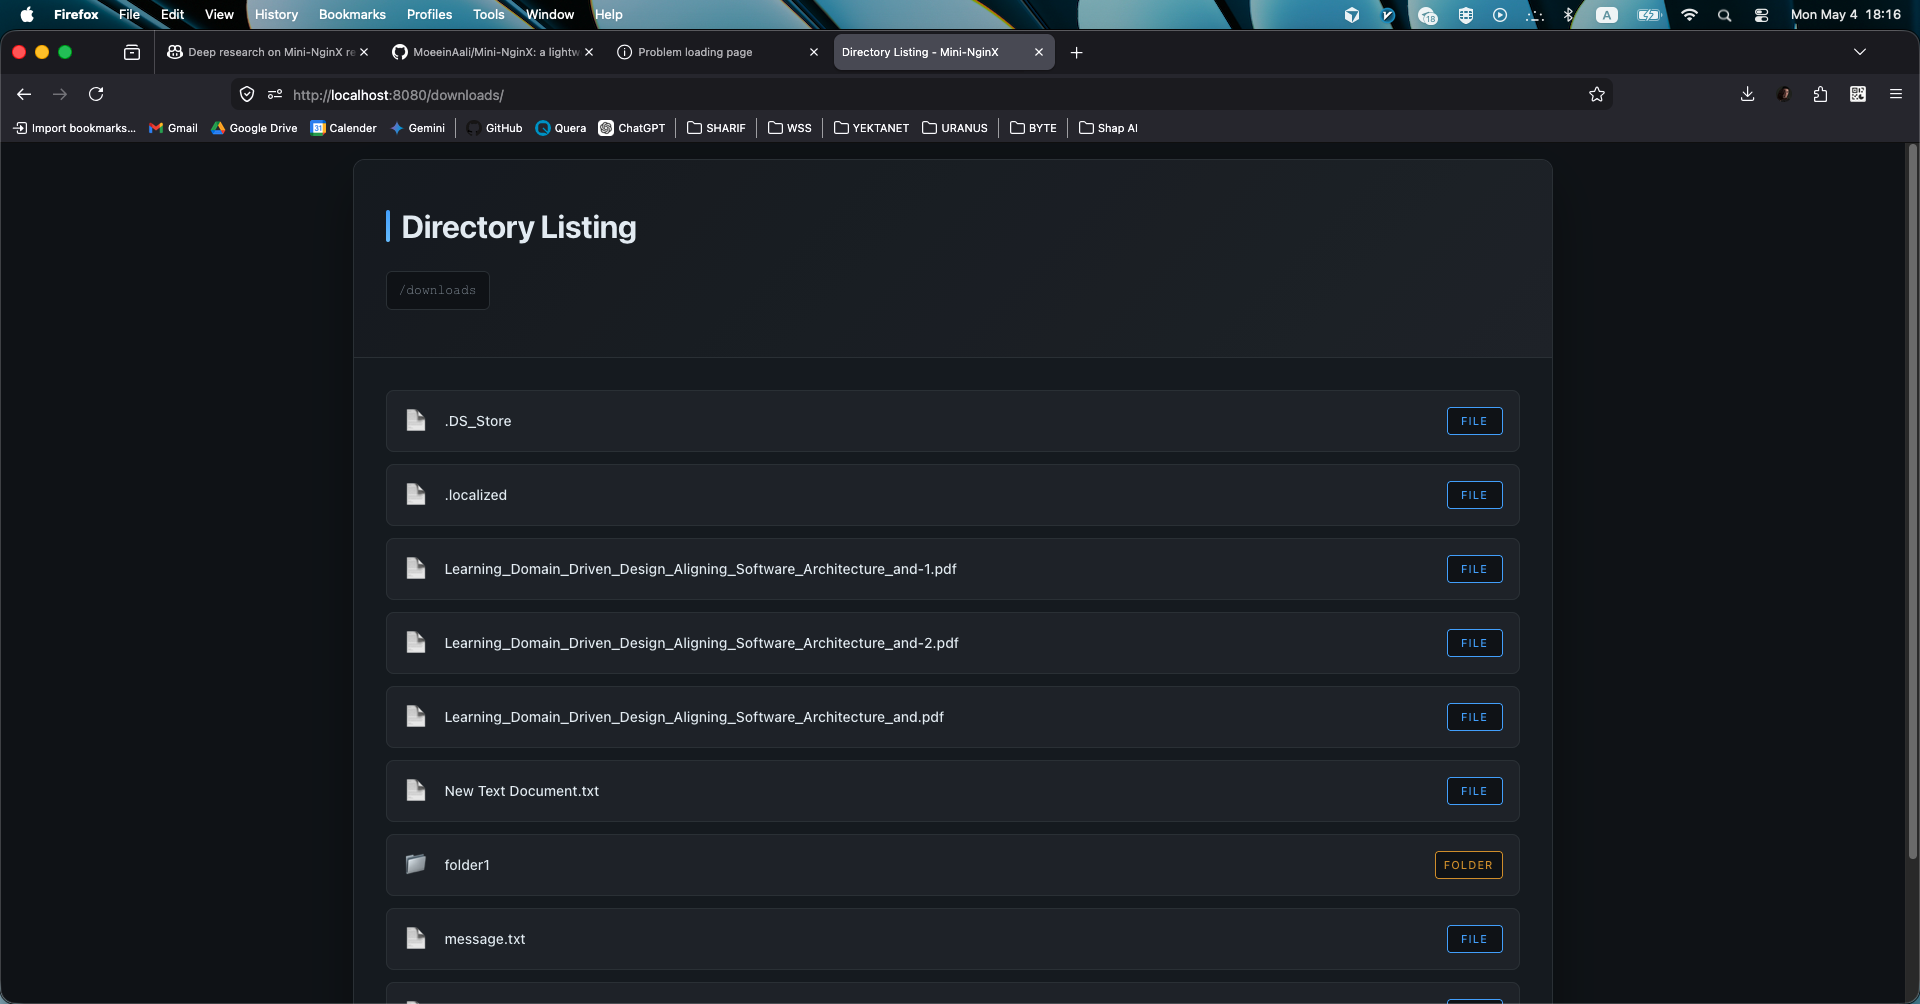
\includegraphics[width=1\textwidth]{figs/downloads1.png}
\end{center}

داخل کانفیگ، مسیر \lr{/downloads} به فولدر دانلودهای سیستم مپ شده. همانطور که در عکس بالا مشخص است، لیست فایل‌ها 
و ساب‌فولدرها و فایل‌ها به درستی سرو شده‌اند. 
با توجه به نوع \lr{MIME} هر فایل، آن را سرو می‌کنیم.
به عنوان مثال هدر ریسپانس فایل‌های \lr{pdf} با \lr{audio} فرق دارد.
همچنین برنامه از سرو فایل‌های داخل ساب‌فولدرها هم پشتیبانی می‌کند.

لاگ‌های پروژه:

\begin{center}
    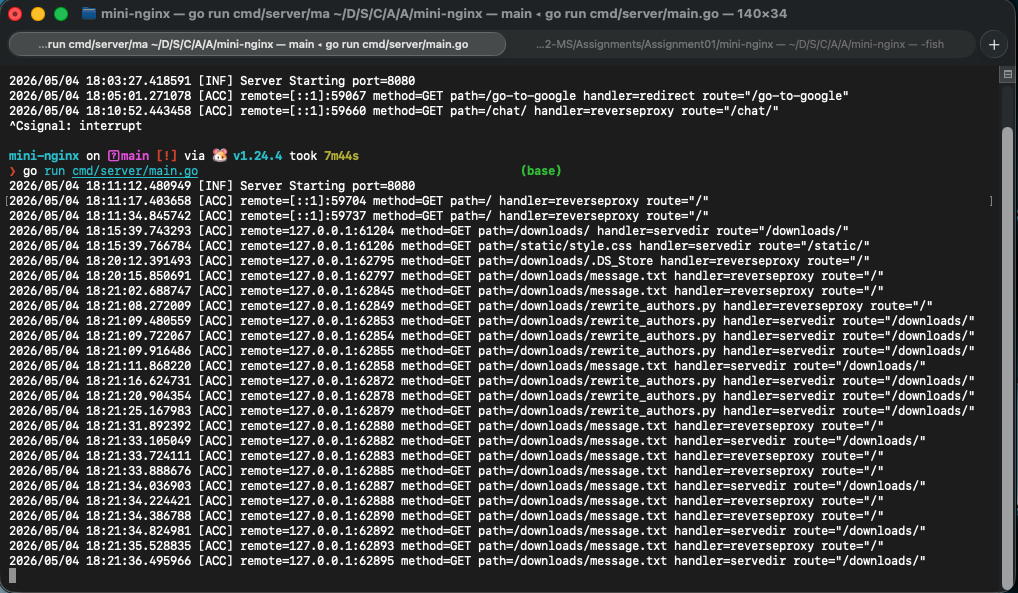
\includegraphics[width=0.5\textwidth]{figs/logging.png}
\end{center}


\subsectionaddtolist{بررسی معماری پروژه و تحلیل کلی}
معماری پروژه \lr{Mini-NginX} بر پایه \lr{Layered Architecture} است، که در آن لایه‌ها به صورت سلسله‌مراتبی سازماندهی شده‌اند تا نگرانی‌ها جدا شوند. این معماری شامل لایه‌های زیر است:

\begin{enumerate}
    \item {لایه Bootstrap :} \texttt{main.go} – بارگذاری تنظیمات و شروع سرور.
    
    \item {لایه Transport :} \texttt{server.go} و \texttt{router.go} – مدیریت اتصالات، پارسیگ درخواست و روتینگ.
    
    \item {لایه منطق برنامه :} \texttt{handlers/*.go} – اجرای استراتژی‌های مختلف برای مسیرها.
    
    \item {لایه Infrastructure :} \texttt{config.go} و \texttt{logger.go} – تنظیمات و لاگینگ.
\end{enumerate}

{دیزاین پترن‌های استفاده‌شده:}
\begin{itemize}
    \item {\lr{Strategy Pattern}:} در لایه \lr{Application} ، با استفاده از \lr{switch} در \texttt{router.go}، رفتار هندلر بر اساس نوع مسیر انتخاب می‌شود. این پترن اجازه می‌دهد استراتژی‌های جدید (مانند هندلر جدید) بدون تغییر کد اصلی اضافه شوند. مثال: اضافه کردن case جدید برای "auth" نیاز به تغییر فقط در switch و پیاده‌سازی هندلر دارد.
    
    \item {\lr{Configuration-as-Code}:} رفتارها در فایل \lr{YAML} تعریف می‌شوند، نه \lr{hardcoded} در کد.
    
    \item {\lr{Dependency Injection}:} شیء \lr{Config} به عنوان پارامتر به لایه‌های پایین‌تر پاس داده می‌شود تا وابستگی‌ها کاهش یابد.
    
    \item {\lr{Concurrency Pattern}:} استفاده از \lr{goroutine per connection} برای پشتیبانی از اتصالات همزمان.
\end{itemize}

معماری و فلوی کلی پروژه \lr{Mini-NginX} به صورت زیر است:

\begin{center}
    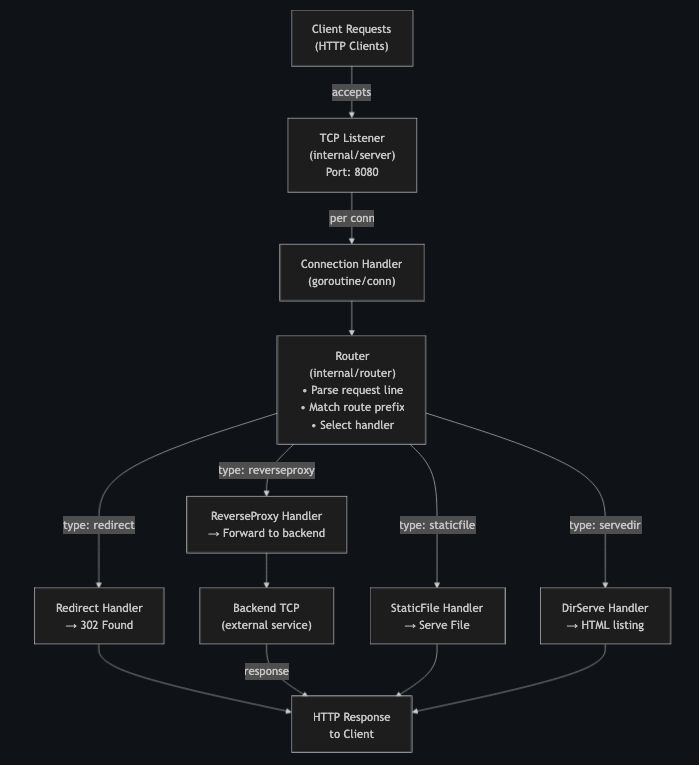
\includegraphics[width=0.6\textwidth]{figs/arch.png}
\end{center}

ساختار فایل‌ها به این صورت است:

\begin{center}
    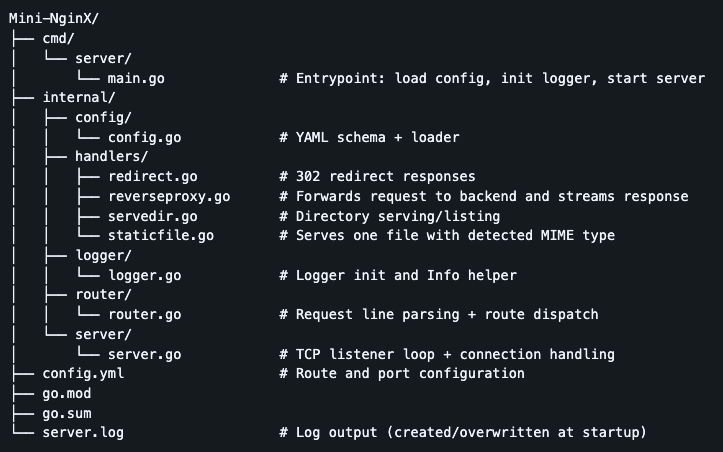
\includegraphics[width=0.7\textwidth]{figs/files.png}
\end{center}


\subsectionaddtolist{قابلیت تغییرپذیری معماری برای اضافه کردن قابلیت جدید}
معماری لایه‌ای پروژه Mini-NginX بسیار تغییرپذیر است، به ویژه به خاطر استفاده از \lr{Strategy Pattern} و جداسازی لایه‌ها.

 برای اضافه کردن قابلیت جدید (مانند هندلر \lr{cache} یا \lr{middleware})، کافی است:
  \begin{enumerate}
      \item نوع جدید را به \lr{YAML} اضافه کنید.
      \item case جدید در switch \texttt{router.go} اضافه کنید.
      \item هندلر جدید در \texttt{handlers/} پیاده‌سازی کنید.
  \end{enumerate}
  این کار بدون تغییر لایه‌های دیگر امکان‌پذیر است و اصل \lr{Open-Closed Principle} رعایت می‌شود.
